%%%%%%%%%%%%%%%%%%%%%%%%%%%%%%%%%%%%%%%%%%%%%%%%%
% Methods
%%%%%%%%%%%%%%%%%%%%%%%%%%%%%%%%%%%%%%%%%%%%%%%%%

\section{Preliminary remark}
It is important to emphasize that principal component analysis and cluster analysis are \emph{exploratory methods} contrary to regression models which predict an outcome. In our work, we separated these two radically different approaches in different chapters. Firstly, we used the exploratory methods in order to summarize the data. Subsequently, we tried to link these findings with hypertension using regression models. The global approach is depicted in Figure \ref{fig:ga}.

\begin{figure}
\centering
\captionsetup{singlelinecheck = false, format= hang, justification=raggedright, font=small, labelsep=space}
\begin{tikzpicture}[node distance=1cm, auto,]
 \node[punkt](reg){Regression models};
 \node[above=of reg](dummy){};
 \node[left=of dummy](if){Individual factors}
edge[pil,bend right=45](reg.west);
 \node[right=of dummy](c){Clusters}
edge[pil,bend left=45](reg.east);
\node[punkt,above=of if](pca){Principal component analysis}
edge[pil,bend left=0](if.north);
\node[punkt,above=of c](ca){Cluster analysis}
edge[pil,bend left=0](c.north);
\node[left=of pca](cara){Participants' characteristics}
edge[pil,bend right=45](reg.west);
\node[above=of pca](dummy2){};
\node[right=of dummy2](me){Biochemical elements}
edge[pil,bend left =10](ca.north)
edge[pil,bend right=10](pca.north);
\end{tikzpicture}
\captionof{figure}{Global approach in our work.}
  \label{fig:ga}
\begin{flushleft}
{\footnotesize  
It is important to emphasize that principal component analysis and cluster analysis are \emph{exploratory methods} contrary to regression models which predict an outcome. In our work, we separated these two radically different approaches in different chapters.}
\end{flushleft}
\end{figure}

\section{Exploratory methods}

%%%%%%%%%%%%%%%%%%%%%%%%%%%%%%%%%%%%%%%%%%%%%%%%%%%%%%%%
%%%%%%%%%%%%%%%%%%%%%%%%%%%%%%%%%%%%%%%%%%%%%%%%%%%%%%%%

\subsection{First method: PCA}
\emph{Principal component analysis} (PCA) is a statistical tool reducing the dimensions of data. This is particularly interesting when the number of variables $p$ is large in order to summarize the information. Basically, we want to project the $p$-dimensional vectors into a $q$-dimension subspace where $q \ll p$. Our summary will be the projection of the original $p$ vectors on to $q$ directions, the principal components (PCs), which span the subspace. A way of deriving the PCs is to find the projections which maximize the variance. The mathematical demonstration we reported below is taken from the book \emph{Advanced Data Analysis from an Elementary Point of View} by Shalizi \cite{pca_book}.

Let $\mathbf{X}$ be a data of size $n \times p$ where $n$ is the number of individuals and $p$ is the number of variables and let $\mathbf{\tilde{X}_c}$ denote the centered reduced data. Let $\mathbf{x_i}$ denote the $i$-th row of $\mathbf{\tilde{X}_c}$. We are looking for the unit vector $\mathbf{w}$ of size $p \times 1$ such that the variance of the projected individuals on it is maximized, i.e. the PC. 

\newpage

The variance is:

\begin{align*}
\hat{\sigma^2} \big ( \overrightarrow{w}\cdot \overrightarrow{x_i} \big ) &= \frac{1}{n} \sum_{i=1}^n \big ( \overrightarrow{x_i}\cdot \overrightarrow{w} \big )^2 \\
&= \frac{1}{n} \big (\textbf{Xw})^T (\textbf{Xw}) \\
&= \frac{1}{n} \textbf{w}^T \textbf{X}^T \textbf{Xw} \\
&= \textbf{w}^T \frac{\textbf{X}^T \textbf{X}}{n} \textbf{w}. \\
\end{align*}

Thus, we want to maximize $\hat{\sigma^2} (\overrightarrow{w}\cdot \overrightarrow{x_i}) $ with the constraint that $\overrightarrow{w} \cdot \overrightarrow{w} =1$. We will use the Lagrangian function with the Lagrange multiplier $\lambda$:

\begin{align*}
\mathcal{L} (\textbf{w},\lambda) & = \textbf{w}^T \frac{\textbf{X}^T \textbf{X}}{n} \textbf{w} - \lambda (\textbf{w}^T \textbf{w} -1) \\
\frac{\partial \mathcal{L}}{\partial \lambda} & = \textbf{w}^T\textbf{w} -1 \\
\frac{\partial \mathcal{L}}{\partial w} & = 2\frac{\textbf{X}^T \textbf{X}}{n} \textbf{w} - 2 \lambda \textbf{w}. \\
\end{align*} 

\newpage

Setting the derivatives to zero, we get:

\begin{align*}
\textbf{w}^T \textbf{w} & = 1 \\
\frac{\textbf{X}^T \textbf{X}}{n} \textbf{w} & = \lambda \textbf{w}. \\
\end{align*}

The solution is given by diagonalization of matrix $\mathbf{\frac{X^T X}{n}}$ which is in fact the covariance matrix. We obtain $p$ eigenvectors $\mathbf{w}$ that are the principal components (PCs)\footnote{also called \emph{loadings}} and $p$ associated eigenvalues $\lambda$. The maximizing vector will be the one associated with the largest eigenvalue $\lambda$. Eigenvalues are directly proportional to the contribution of their associated PC to the total variance. By nature of diagonalization, the PCs are orthogonal to each other.

All individuals and variables can then be projected on the PCs in order to find some homogeneous patterns of variables or individuals in the data. These projections are called \emph{factors} or \emph{scores}.

Other PCA results are:
\begin{itemize}
\item \emph{Cosine}: the correlation between the variable and the factor \cite{tille_multivariate_nodate},
\item \emph{Squared cosine}: measures the quality of the representation of the variable by a factor \cite{tille_multivariate_nodate}.
\end{itemize}

Following the methodology of Pang et al., we performed a PCA on all urine element excretions \cite{pang_metal_2016}. Before running the PCA, we standardized the variables to unit variance and zero mean.

Using the Elbow method, we selected the first 3 PCs. The Elbow method consists in finding the eigenvalues that are on the left of the line that separates the rapidly decreasing eigenvalues and the approximately equal eigenvalues (Figure \ref{fig:elbow}) \cite{abdi_principal_2010}. Another method for significant PC selection is to select all principal components with eigenvalues greater than 1 \cite{tille_multivariate_nodate}. Using the latter method in this study would mean selecting 7 PCs, which is excessive. As shown by Trevor Hastie et al., we computed the eigenvalues on a normally simulated data $X_{sim}$ of the same dimension as $\tilde{X}_c$, with all $n\cdot p$ cells with unit variance and zero mean \cite{james_introduction_2013}. Values from the simulated data are represented by blue crosses in Figure \ref{fig:elbow}. Only the first 3 eigenvalues are bigger than the simulated ones, which brings us to the same conclusion as for the Elbow method.

\begin{figure}
\centering
\captionsetup{singlelinecheck = false, format= hang, justification=raggedright, font=small, labelsep=space}
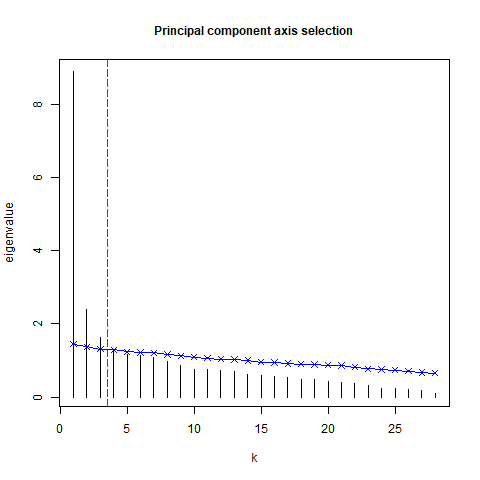
\includegraphics[width=0.45\linewidth]{elbow}
\captionof{figure}{Selecting significant principal components.}
  \label{fig:elbow}
\begin{flushleft}
{\footnotesize  Using the Elbow method, we selected the first 3 principal components. The Elbow method consists in finding the eigenvalues that are on the left of the line that separates the rapidly decreasing eigenvalues and the approximately equal eigenvalues (red line). Eigenvalues from normally simulated data are represented by blue crosses. Only the first 3 eigenvalues are bigger than the simulated ones.}
\end{flushleft}
\end{figure}

%%%%%%%%%%%%%%%%%%%%%%%%%%%%%%%%%%%%%%%%%%%%%%%%%%%%%%%%
%%%%%%%%%%%%%%%%%%%%%%%%%%%%%%%%%%%%%%%%%%%%%%%%%%%%%%%%

\subsection{Second method: cluster analysis}
In this section, we will firstly introduce some general considerations on clustering methods and distance metrics. Afterwards, we will describe the three main steps we followed to construct our clusters:
\begin{enumerate}
\item Computing a \emph{distance matrix}: the Manhattan matrix \cite{hennig_handbook_2016},
\item Choosing a clustering algorithm: the PAM algorithm \cite{hennig_handbook_2016},
\item Selecting the number of clusters: the silhouette index \cite{hennig_handbook_2016,kaufman_finding_1990}.
\end{enumerate}

\subsubsection{General considerations on clustering methods}
\emph{Cluster analysis} is a method of finding homogeneous groups in data \cite{kaufman_finding_1990}. These groups are called \emph{clusters}. The number of clusters $K$ is either chosen in function of cluster validation indexes (\emph{parametric clustering}) or itself determined by the clustering method (\emph{nonparametric clustering}) \cite{hennig_handbook_2016}. Clustering methods are unsupervised methods since their aim is not to predict a response variable. After clustering, members assigned to the same cluster are expected to be close to each other in the $p$-dimension space. If the $p$ variables are continuous, this proximity can be defined in terms of Euclidean distance. However other distance metrics exist: the Minkowski-type distance, the Hausdorff distance, the Mahahanobis distance, the Gower dissimilarity, etc \cite{hennig_handbook_2016}. Cluster analysis should not be confused with linear discriminant analysis. Whereas the aim of clustering methods is to establish groups, the aim of linear discriminant analysis is to assign individuals to groups which are already established \cite{hennig_handbook_2016,tille_multivariate_nodate}.

Different types of distances are:
\begin{enumerate}
\item \textbf{Standard Euclidean distance}. If $p$ is the number of variables, the standard Euclidean distance between individuals $x_i$ and $x_j$ and denoted by $d(x_i,x_j)$ is given by:
\begin{equation*}
d(x_i,x_j)=\sqrt{\sum_{l=1}^p (x_{il} - x_{jl} )^2},
\end{equation*}
where $x_{il}$ and $x_{jl}$ are the values taken in variable $l$ by individuals $x_i$ and $x_j$, respectively.
\item \textbf{Manhattan distance}. If $p$ is the number of variables, the Manhattan distance between individuals $x_i$ and $x_j$ and denoted by  $d(x_i,x_j)$ is given by:
\begin{equation*}
d(x_i,x_j)=\sum_{l=1}^p \mid x_{il} - x_{jl} \mid,
\end{equation*}
where $x_{il}$ and $x_{jl}$ are the values taken in variable $l$ by individuals $x_i$ and $x_j$, respectively.

Instead of taking the square of the differences, we are taking the absolute value of the differences. This distance is typically used when adding one unit to $x_{i1}$ and one unit to $x_{i2}$ is the same than adding two units to $x_{i1}$ for any individual $i$ \cite{kaufman_finding_1990}.
\item \textbf{Minkowski distance}. The Euclidean and the Manhattan distances are special cases of the so-called Minkowski distance where $q=2$ for Euclidean distance and $q=1$ for Manhattan distance in the formula below. If $p$ is the number of variables, the Minkowski distance between individuals $x_i$ and $x_j$ and denoted by $d(x_i,x_j)$ is given by:
\begin{equation*}
d(x_i,x_j)= \Big ( \sum_{l=1}^p \mid x_{il} - x_{jl} \mid^q \Big )^{1/q},
\end{equation*}
where $x_{il}$ and $x_{jl}$ are the values taken in variable $l$ by individuals $x_i$ and $x_j$, respectively \cite{hennig_handbook_2016}.
\item \textbf{Gower dissimilarity}. When the Euclidean and the Manhattan distances are distance metrics for continuous variables, the so-called \emph{Gower dissimilarity} allows to aggregate $p$ variables of mixed type. If the data does not contain any missing value the Gower dissimilarity between individuals $x_i$ and $x_j$ and denoted by  $d_G(x_i,x_j)$ is given by:
\begin{equation*}
d_G(x_i,x_j) = \frac{\sum_{l=1}^p w_j \cdot d_l(x_{il},x_{jl})}{\sum_{j=1}^p w_j},
\end{equation*}
where $d_l(x_{il},x_{jl})$ is the Manhattan distance between individuals $x_i$ and $x_j$ for variable $l=1,2\dots p$ \cite{hennig_handbook_2016}. As reported by Hennig et al., Gower recommended to use weights $w_l$ to scale the distances for each variable between 0 and 1 such that $w_j\cdot d_l(x_il,x_jl) \in [0,1]$ for all possible pairs of $x_j$ and $x_j$ individuals. However, Hennig et al. argued to reserve them only for binary and ``very discrete variables'' because otherwise the weights could have an excessive high influence on the cluster borders. Hennig et al. also said that weights may be used in order to give more importance to some variables that are considered as main variables \cite{hennig_handbook_2016}.
\end{enumerate}

\subsubsection{Clustering procedure}

\paragraph{First step: computing the distance matrix.}
The Manhattan distance matrix is computed between all the individuals taking into consideration all standardized urine excretions. The result can then be presented as a $n \times n$ distance matrix. In our case, the distance matrix has dimension $608 \times 608$. The function \texttt{daisy()} from the \texttt{cluster} packcage in \texttt{R} computes the distance matrix. In one-line code we obtained our Manhattan distance matrix:
\begin{verbatim}
mydaisy<-daisy(...,metric = "manhattan")
\end{verbatim}

\paragraph{Second step: choosing a clustering algorithm (PAM).}
The heuristic \emph{partitioning around medoids} (PAM) algorithm belongs to the $k$-medoids clustering methods. The idea behind $K$-medoids is not dissimilar to that of $k$-means. However, whilst we are sampling random points in the $p$-dimension space in $k$-means, we are sampling existing points in $k$-medoids. Compared to $k$-means clustering, this is often a more robust method since it generally does not consider the squared Euclidean distance which is very sensitive to extreme outliers. PAM is an \emph{hard} clustering method. In \emph{hard} clustering, members are assigned to a precise cluster $k$ with null probability of belonging to the $K-1$ remaining clusters. In contrast, in \emph{soft} clustering every member has a degree of membership to each $K$ cluster \cite{hennig_handbook_2016}.

\newpage

The PAM algorithm follows the procedure described in the book \emph{Handbook of Cluster Analysis} by C. Hennig et al. 2016 \cite{hennig_handbook_2016} in five steps:
\begin{displayquote}
\begin{enumerate}
\item Initialize: randomly select (without replacement) $K$ of the $N$ data points as the initial medoids\footnote{However, Kaufman et al. recommend to take non-random data points as the initial medoids \cite{kaufman_finding_1990}.}.
\item Assign each observation to the medoid with which it is closest, where closest is based on a specific distance measure and compute the total cost across all observations, where the cost is the sum of the distance of each observation to its associated medoid.
\item For each medoid $k$, for $k=1$,\dots ,$K$ consider all $N-K$ nonmedoid, $o$. Swap $k$ and $o$ and recompute the total cost.
\item Select the solution with the lowest cost.
\item Repeat steps 2-4 until the set of medoids does not change.
\end{enumerate}
\end{displayquote}

Finding the $K$ medoids is an optimizing problem with a globally optimal solution since we have a finite number of ${N}\choose{K}$ candidate solutions. However, computational cost is often huge in practice. For example, for $N=500$ and $K=5$ which is a realistic example in practice, we would have $2\cdot 10^{11}$ possible sets of medoids and thus $2\cdot 10^{11}$ costs to compute. With the PAM algoritm, only $K \cdot (N-K)$ costs are computed during the first iteration (2475 in our example).

Let us take a simple example to illustrate the PAM algorithm with $n=10$ individuals and 2 variables, $x$ and $y$. Our objective will be to construct two clusters ($K=2$). This data was generated by \texttt{R}:
\begin{verbatim}
set.seed(123)
data<-runif(20)
x<-data[1:10]
y<-data[11:20]
\end{verbatim}

The data is presented in Table \ref{table:dataex}. The corresponding Euclidean distance matrix is shown in Table \ref{table:distmex}. The first iteration of a $k$-medoids algorithm is shown in Figure \ref{fig:pamex2}. In step 1, observations 7 and 9 are randomly chosen as medoids $m_1$ and $m_2$, respectively. In step 2, the sum of the distances is computed in this configuration, assigning the non-medoids to their closest medoid ($\text{cost}_0 = 2.97$). In steps 3 and 4, $m_1$ is swapped with observation 1 as this decreases the sum of the distances by -1.59. Steps 2-4 are repeated until medoid stabilization is achieved. See the \emph{Appendix} for the PAM program used to solve this example.

\begin{table}
\centering
\captionof{table}{Example data for a $k$-medoids algorithm.}
\begin{tabular}{p{2.5cm} p{2cm} p{2cm} }
\toprule
ID & x & y \\
\midrule
\input{dataex.txt}
\bottomrule
\end{tabular}
\label{table:dataex}
\end{table}

\begin{table}
\centering
\captionof{table}{Distance matrix for the example given in Table 4.1.}
\begin{tabular}{ r | rrrrrrrrr}
\toprule
     & 1  &  2  &  3  &  4   & 5  &  6  &  7    &8  &  9 \\
\midrule
2&  0.71      \\                                   
3 & 0.30& 0.44        \\                            
4  &0.71& 0.15& 0.49       \\                        
5 & 1.07 &0.38 &0.78& 0.47    \\                     
6 & 0.25& 0.87& 0.43& 0.90 &1.20       \\              
7 & 0.75& 0.33& 0.45 &0.48& 0.44& 0.81        \\
8 & 1.10 &0.42& 0.80 &0.53& 0.08&1.21 &0.42           \\
9 & 0.68 &0.27& 0.38 &0.41& 0.45&0.76 &0.09 &0.44      \\
10& 0.17& 0.60& 0.28 &0.57& 0.98 &0.41 &0.71 &1.01& 0.63 \\
\bottomrule
\end{tabular}
\label{table:distmex}
\end{table}

\begin{figure}
\captionsetup{singlelinecheck = false, format= hang, justification=raggedright, font=small, labelsep=space}
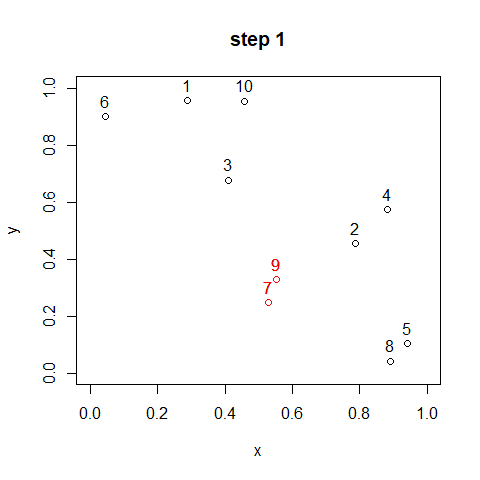
\includegraphics[width=0.45\linewidth]{pamex_s1} \hfill
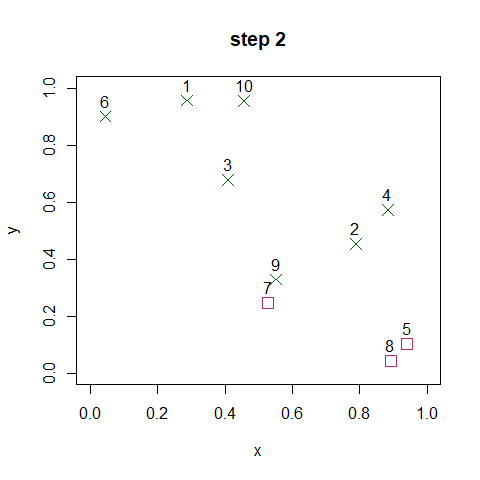
\includegraphics[width=0.45\linewidth]{pamex_s2} \\
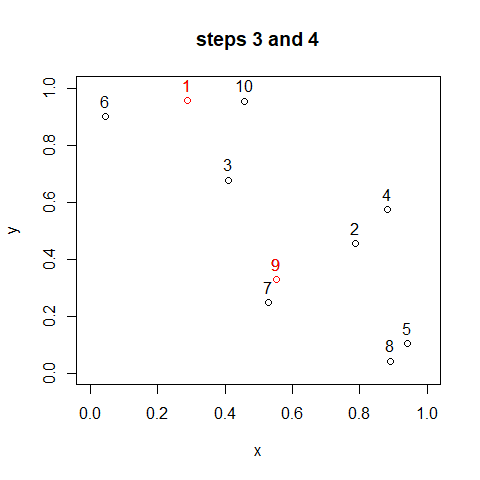
\includegraphics[width=0.45\linewidth]{pamex_s3} \hfill
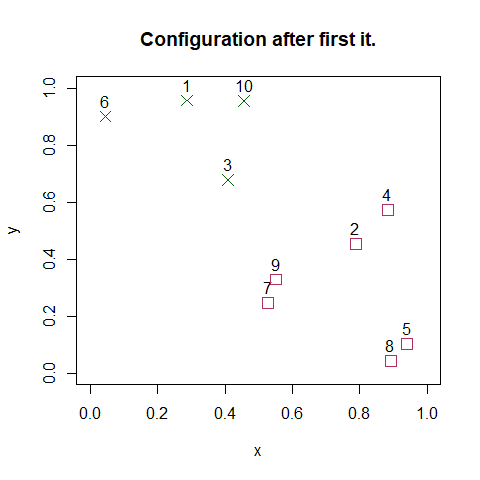
\includegraphics[width=0.45\linewidth]{pamex_s4} \\
\captionof{figure}{First iteration of the algorithm for the example given in Table 4.1.}
\label{fig:pamex2}
{\footnotesize In \textbf{step 1}, observations 7 and 9 are randomly chosen as medoids $m_1$ and $m_2$, respectively. In \textbf{step 2}, the sum of the distances is computed in this configuration, assigning the non-medoids to their closest medoid ($\text{cost}_0 = 2.97$). In \textbf{steps 3 and 4}, $m_1$ is swapped with observation 1 as this decreases the sum of the distances by -1.59. Steps 2-4 are repeated until medoid stabilization is achieved.}
\end{figure}

The PAM algorithm was implemented with SKIPOGH data using the \texttt{pam()} function from the \texttt{cluster} package in \texttt{R} \cite{rblog}.

\paragraph{Third step: selecting the number of clusters.}
To select the optimal number of clusters, we computed the \emph{silhouette index}, also called \emph{silhouette width}, for $K=1,2,\dots 10$. The number of clusters $K$ associated with the biggest silhouette index was selected. The silhouette index $SI_K$ is defined as \cite{kaufman_finding_1990}:
\begin{equation*}
SI_K = \frac{1}{n} \sum_{i=1}^n \frac{b(i)-a(i)}{max\{a(i),b(i)\}},
\end{equation*}
where $a(i)$ is the average dissimilarity between object $i$ and all objects in its cluster and $b(i)$ is the minimum average dissimilarity of $i$ to all points in any other cluster not including $i$ \cite{hennig_handbook_2016}. In our work we used the Manhattan dissimilarity. The silhouette index is bounded between minus one and one, i.e. $SI_K \in [-1,1]$.

\newpage

As reported by Struyf et al. \cite{JSSv001i04}, the value $SI_K$ may be interpreted as follows:

\begin{displayquote}
\begin{itemize}
\item $SI_K \approx 1 \Rightarrow$ object $i$ is well classified (in $A$),
\item $SI_K \approx 0 \Rightarrow$ object $i$ lies intermediate between two clusters ($A$ and $B$),
\item $SI_K \approx -1 \Rightarrow$ object $i$ is badly classified (closer to $B$ than to $A$).
\end{itemize}
\end{displayquote}

Thus, the higher the index is, the more distinguishable the clusters are. Conceptually, the silhouette index measures the distance between the clusters whilst taking into account out each cluster is (see examples in Figure \ref{fig:silex}). Not only can the silhouette index be used as a tool to chose the optimal number of clusters, but also to measure the quality of the clustering result and thereby is an index for cluster validation.

\begin{figure}
\captionsetup{singlelinecheck = false, format= hang, justification=raggedright, font=small, labelsep=space}
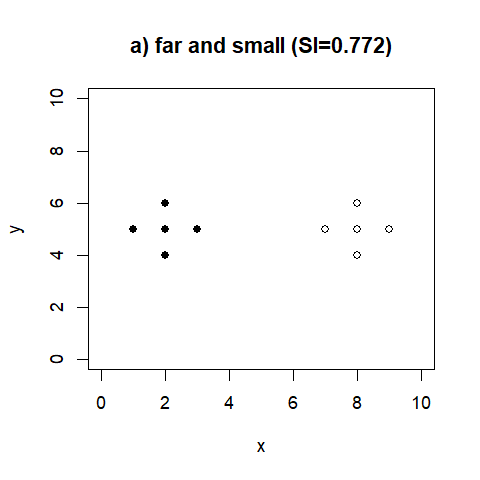
\includegraphics[width=0.45\linewidth]{siex1} \hfill
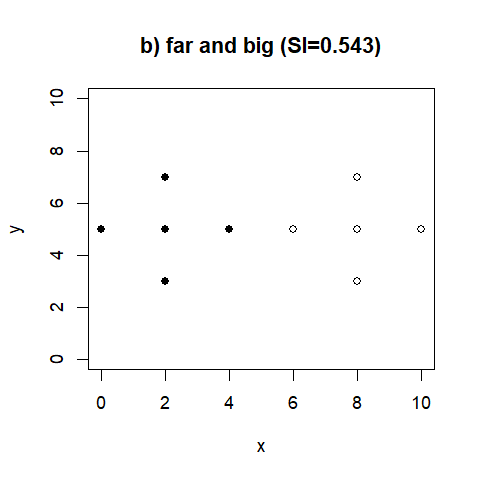
\includegraphics[width=0.45\linewidth]{siex2} \\
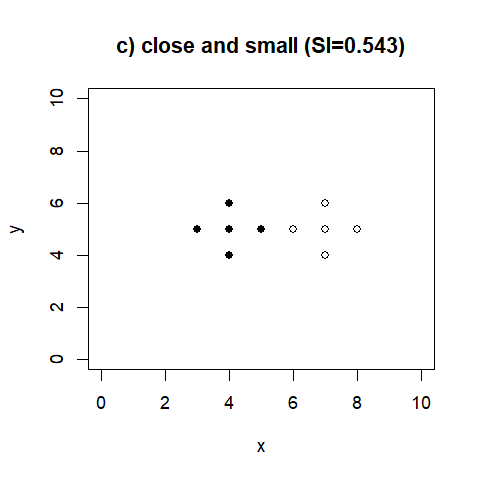
\includegraphics[width=0.45\linewidth]{siex3} \hfill
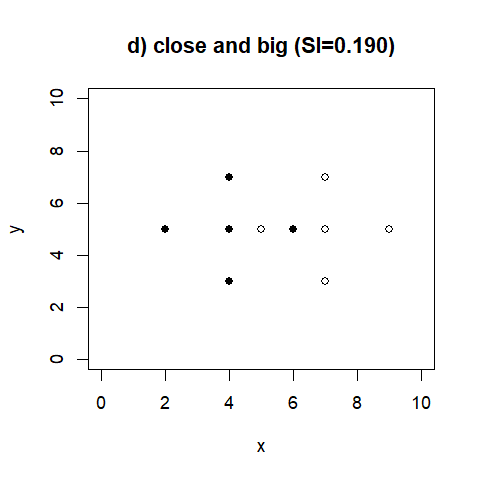
\includegraphics[width=0.45\linewidth]{siex4} \\
\captionof{figure}{Examples of silhouette index.}
\label{fig:silex}
{\footnotesize These plots show 4 situations concerning 2 clusters (white and black). They illustrate that the silhouette index takes into consideration both the size of the clusters and the distance between each other. Plot a) where the clusters are far and small has the highest silhouette index ($SI_K=0.772$). Plot b) where the clusters are far and big and plot c) where the clusters are close and small have the same silhouette index ($SI_K=0.543$). Plot d) where the clusters are close and big has the lowest silhouette index ($SI_K=0.190$).}
\end{figure}

%%%%%%%%%%%%%%%%%%%%%%%%%%%%%%%%%%%%%%%%%%%%%%%%%%%%%%%%
%%%%%%%%%%%%%%%%%%%%%%%%%%%%%%%%%%%%%%%%%%%%%%%%%%%%%%%%

\section{Assessing for cluster stability}
If we state that our data is a random sample from a finite population, we can consider clustering as a random process. In this scope, clusters are random. However, we would like to construct $K$ clusters from our data that are the more stable as possible. In order to assess for cluster stability, we will summary two methods:

\begin{enumerate}
\item \textbf{The Rand index} \cite{rand_objective_1971}. The \emph{Rand index} is a measure of cluster stability. Firstly, we divide the data of dimension $n \times p$ into three parts: two training sets $S$ and $T$ and one testing set $E$. Then, we perform a clustering on $S$ giving $\mathcal{C}_S$ and on $T$ giving $\mathcal{C}_T$, independently. The purpose is to use points of $E$ to see if there is a difference in cluster attribution if we are using the medoids of $\mathcal{C}_S$ or the medoids of $\mathcal{C}_T$. The rand index is given by:
\begin{equation*}
\mathcal{R}(\mathcal{C}_S,\mathcal{C}_T)=\frac{N_{11}+N_{00}}{n(n-1)/2},
\end{equation*}

where $N_{11}$ is the number of point pairs of $E$ that are in the same cluster with both $\mathcal{C}_S$ and $\mathcal{C}_T$ and where $N_{00}$ is the number of point pairs of $E$ in different clusters with both $\mathcal{C}_S$ and $\mathcal{C}_T$ \cite{hennig_handbook_2016}.

Since Rand index is random from the sampling step, a bootstrap version combining a kind of Rand index and bootstrap techniques was described by Dolnicar and Leisch in 2010 \cite{dolnicar_evaluation_2010}.

\item \textbf{Bootstrapping average cluster stability} \cite{dolnicar_evaluation_2010}. The technique computes several replicates of Rand indices with the notable difference that $S_i$ and $T_i$ are both bootstrapped samples of size $n$ from the original data that replace $S$ and $T$ in the classical Rand index. The formula for the replicates is:

\begin{equation*}
\mathcal{R}_i(\mathcal{C}_{S_i},\mathcal{C}_{T_i})=\frac{N_{{11}_i}+N_{{00}_i}}{n(n-1)/2},
\end{equation*}
where $N_{{11}_i}$ is the number of point pairs of $E$ that are in the same cluster under both $\mathcal{C}_{S_i}$ and $\mathcal{C}_{T_i}$ and where $N_{{00}_i}$ is the number of point pairs of $E$ in different clusters under both $\mathcal{C}_{S_i}$ and $\mathcal{C}_{T_i}$ \cite{dolnicar_evaluation_2010}. The mean and the standard deviations of bootstrapped replicates are estimates of expectation and standard error of Rand index, respectively.
\end{enumerate}

%%%%%%%%%%%%%%%%%%%%%%%%%%%%%%%%%%%%%%%%%%%%%%%%%%%%%%%%
%%%%%%%%%%%%%%%%%%%%%%%%%%%%%%%%%%%%%%%%%%%%%%%%%%%%%%%%

\section{Checking for assumptions}
Statistical test results are not presented if assumptions are violated. For every performed two-sided two-sample Student’s test, normality in the two groups was assessed using normal Q-Q plots. Moreover, equal variance assumption was adopted if the $p$-value in the Levene's test was larger than $5\%$.

